\chapter[Struttura aziendale e del suo \texttt{SI}]{La struttura dell’azienda e del suo sistema informativo}
\thispagestyle{chapterInit}
In questo capitolo verrà analizzato il concetto di \textbf{esigenza informativa} e verranno trattati i sistemi operazionali e informativi.
\section{Concetto di esigenza informativa}
    \paragraph{Funzione \texttt{SI}} La funzione primaria del \textbf{sistema informativo} è quella di aiutare e guidare chi svolge mansioni che mandano avanti l'azienda attraverso queste. Inoltre il \texttt{SI} deve essere di aiuto e guida in modo diverso per aree diverse, ciò tramite il \textbf{livello d'astrazione} che sale man mano che si sale di livello gerarchico. L'\textbf{esigenza informativa} dipende dal tipo di attività svolta e dal livello gerarchico dell'utente. (es. i livelli operativi hanno bisogno di informazioni attuali ed precise spesso il singolo dato, mentre i livelli direzionali hanno bisogno di informazioni sintetizzate anche su periodi più lunghi).
    \subsubsection{Schema di Anthony}
        \label{subsec:schemaAnthony}
        L'organizzazione aziendale è vista a forma piramidale con i livelli operativi alla base, i livelli intermedi al centro e i livelli direzionali in cima. Ogni livello ha bisogno di informazioni diverse e quindi il \texttt{SI} deve essere in grado di fornire informazioni adeguate a ciascun livello.
        \begin{figure}[H]
            \centering
            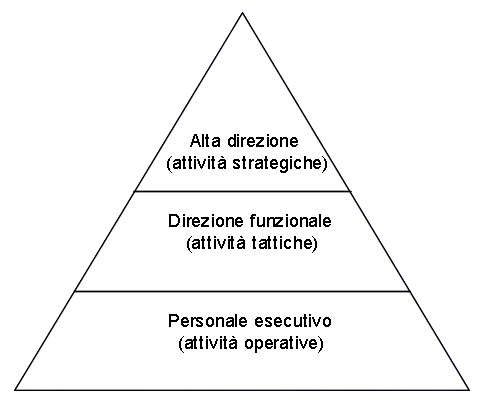
\includegraphics[width=0.4\textwidth]{03/schemaAnthony.png}
            \caption{Schema di Anthony}
        \end{figure}
    \subsubsection{Profili Informativi}
        Di seguito è riportata una tabella con i profili informativi di ciascun livello, si può notare come i livelli operativi abbiano bisogno di poche informazioni ma molto dettagliate, precise e in modo continuo, il livello direzionale tattico ha accesso ai dati con frequenza minore ma prefissata e con un livello di dettaglio minore produce quindi un volume medio di informazioni, il livello strategico ha bisogno di informazioni molto sintetizzate e con una frequenza molto bassa se non sporadica ma ha bisogno anche di informazioni esterne all'azienda.
        \begin{table}[H]
            \begin{adjustbox}{width=\textwidth}
                \begin{tabular}{|c|c|c|c|c|}
                    \hline
                    & \textbf{Frequenza} & \textbf{Dati} & \textbf{Provenienza dati} & \textbf{Volume} \\
                    \hline
                    \textbf{Livello direzionale strategico} & Sporadica & molto sintetizzati & interni ed esterni & basso \\
                    \hline
                    \textbf{Livello direzionale tattico} & Prefissata & sintetici e analitici & interni & medio \\
                    \hline
                    \textbf{Livello operativo} & Continua & analitici & interni & elevati \\
                    \hline
                \end{tabular}
            \end{adjustbox}
        \end{table}
\section{Scomposizione dei sistemi informativi}
    Le diverse esigenze informative, dei vari livelli gerarchici, hanno portato ad una separazione delle funzioni decisionali e operative in due tipi di sistemi informativi: quelli orientati al supporto operativo e quelli orientati alle decisioni. Spesso i sistemi orientati al supporto operativo hanno delle funzioni di \textit{reporting} che si avvicinano a quelle dei sistemi orientati alle decisioni ma vista la necessità di rapidità e precisione delle informazioni per i livelli decisionali e tattici è sorta la necessità di sviluppare sistemi informativi direzionali.

    \subsection{Sistemi operazionali}
        I sistemi operazionali sono sistemi che permettono di raccogliere, elaborare e presentare informazioni utili per il supporto delle attività operative dell'azienda. Questi sistemi sono orientati a supportare le attività di esecuzione e controllo delle operazioni aziendali e dunque sono usati dai livelli operazionali e dalla direzione funzionale.
        \textit{On Line Transaction Processing} (\texttt{OLTP}) è un termine usato per descrivere un'attività di gestione dei dati che permette di svolgere attività operative. Questi sistemi permettono di gestire i dati in modo operativo e di automatizzare le attività aziendali.
        \paragraph{Funzioni principali}
            \begin{itemize}
                \item Automazione di attività procedurali - In questo caso il \texttt{SI} è un supporto all'operatore
                \item Definizione di nuovi processi - come visto sottosezione \ref{subsec:nuoviProcessi}
                \item Aiuto nelle attività aziendali 
                \item Raccolta di dati - gli operatori inseriscono i dati nel sistema in modo continuo
                \item Guida per l'operatore - il sistema guida l'operatore nelle attività da svolgere in questo modo si riducono gli errori
            \end{itemize}
        \paragraph{Azioni sui dati}
            \begin{itemize}
                \item Accesso interattivo in inserimento, lettura, modifica - l'operatore può interagire con il sistema e modificare i dati nei limiti imposti 
                \item Trattamento di dati - il sistema tratta i dati in modo automatico e li presenta all'operatore in modo chiaro 
                \item Descrizione di eventi - il sistema descrive le transazioni e le attività svolte in modo da poterle ripetere in caso di necessità
                \item Valutazione e trattamento di informazioni utili - il sistema valuta i dati se sussistono errori e li segnala all'operatore
                \item Aggregazione per il calcolo di indicatori di stato - il sistema aggrega i dati per calcolare indicatori di stato dell'azienda
            \end{itemize}
        \paragraph{Componenti fondamentali}
            \begin{itemize}
                \item Base si dati operazionale - contiene i dati operativi dell'azienda
                \item Funzioni operative - funzioni che permettono di svolgere le attività operative
            \end{itemize}
    \subsection{Sistemi informazionali}
        I sistemi informazionali (o direzionali) sono sistemi che permettono di raccogliere, elaborare e presentare informazioni utili per il processo decisionale. Questi sistemi sono orientati a supportare le attività di controllo e di pianificazione dell'azienda e dunque sono usati dai livelli dell'alta direzione e dalla direzione funzionale. 
        \textit{On Line Analytical Processing} (\texttt{OLAP}) è un termine usato per descrivere un'attività di analisi dei dati che permette di estrarre informazioni utili per il processo decisionale. Questi sistemi permettono di analizzare i dati in modo multidimensionale e di presentarli in modo chiaro e comprensibile.
        \paragraph{Funzioni principali}
            \begin{itemize}
                \item Facilitazione del processo decisionale
                \item Presentazione dei dati secondo diverse aggregazioni e viste
                \item Confronto tra indicatori aziendali e indicatori esterni
            \end{itemize}
        \paragraph{Azioni sui dati}
            \begin{itemize}
                \item Accesso in lettura
                \item Aggregazione dei dati
                \item Descrizione di aree/temi
                \item Profondità temporale
                \item Multi-dimensionalità
            \end{itemize}
        \paragraph{Componenti fondamentali}
            \begin{itemize}
                \item Base dati informativa
                \item Strumenti di analisi
                \item Procedure di alimentazione (dati)
            \end{itemize}
    \subsection{Comparazione}
        \begin{table}[H]
            \begin{adjustbox}{width=\textwidth}
                \begin{tabular}{|c|c|c|}
                    \hline
                    & \textbf{Operazionale} (\texttt{OLTP}) & \textbf{Informazionale} (\texttt{OLAP}) \\
                    \hline
                    \textbf{Finalità} & Supporto all'operatività & Supporto alle decisioni \\
                    \hline
                    \textbf{Utenti} & Molti, operativi & Pochi, direzionali \\
                    \hline
                    \textbf{Dati} & Dettagliati, transazionali & Sintetici, aggregati \\
                    \hline
                    \textbf{Modo d'uso} & Guidata (Operazioni predeterminate) & Interrogazioni ad hoc \\
                    \hline
                    \textbf{Quantità dati per attività elementare} & Pochi record & Molti record \\
                    \hline
                    \textbf{Orientamento} & Per processo & Per area \\
                    \hline
                    \textbf{Frequenza aggiornamento} & Continuo & Periodica se non sporadica \\
                    \hline
                    \textbf{Copertura temporale} & Breve & Lunga \\
                    \hline
                    \textbf{Ottimizzazione} & Per accessi in scrittura & Per accessi in lettura \\
                    \hline
                \end{tabular}
            \end{adjustbox}
        \end{table}